\chapter{Modelo de Persistencia y Acceso a Datos}
\label{cap:persistencia}
%---------------------------------------------------------
\section{Modelo de Persistencia y Acceso a Datos}

\subsection{Modelo Relacional}
    
    \begin{figure}[htbp!]
    	\begin{center}
    		\fbox{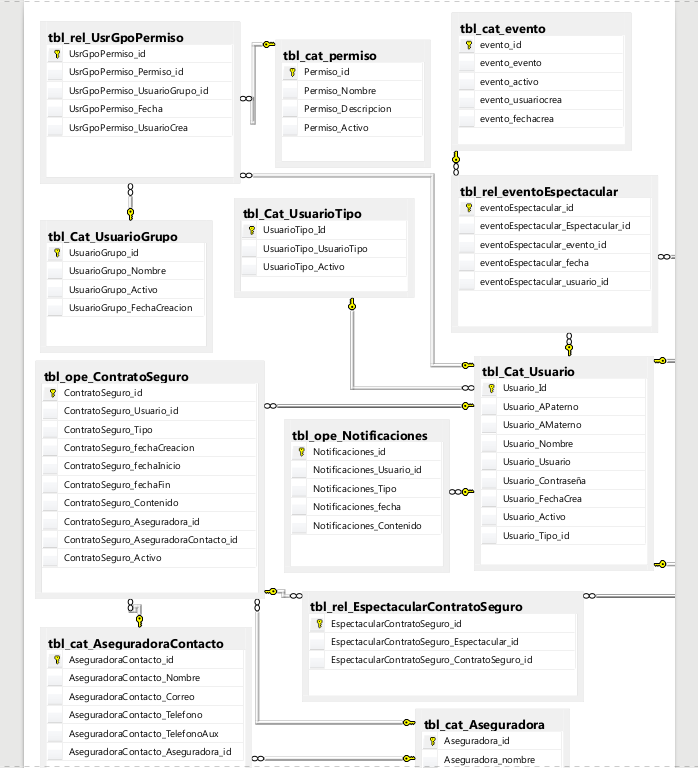
\includegraphics[width=.7\textwidth]{tlato-images/diag1}}
    		\caption{Parte 1 del diagrama Relacional}
    		\label{fig:diag1}
    	\end{center}
    \end{figure}
    \begin{figure}[htbp!]
    	\begin{center}
    		\fbox{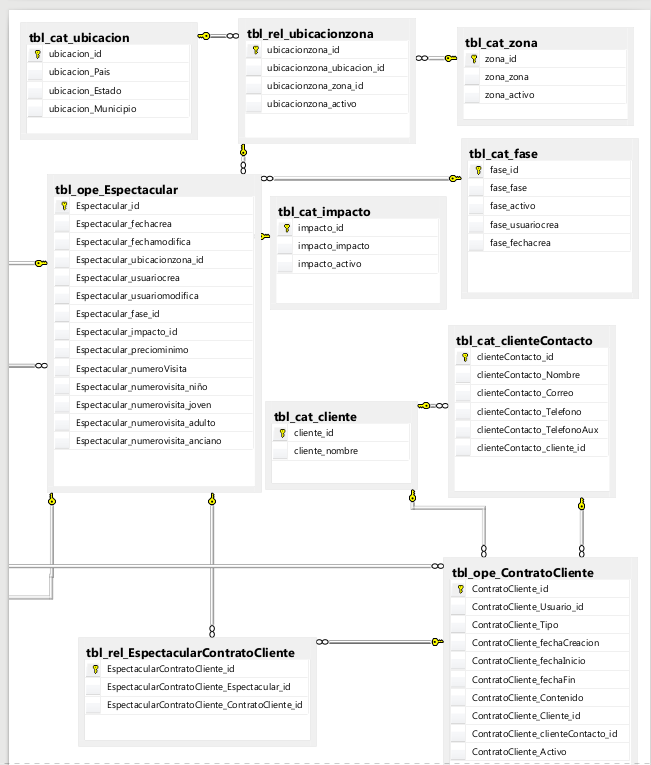
\includegraphics[width=.7\textwidth]{tlato-images/diag2}}
    		\caption{Parte 2 del diagrama Relacional}
    		\label{fig:diag2}
    	\end{center}
    \end{figure}
    
    En las figuras~\ref{fig:diag1} y ~\ref{fig:diag2} se muestra completa la arquitectura del modulo de persistencia de datos.
    
    Se muestran los campos de cada tabla, donde cada nombre es muy específico, haciendo fácil el que se entienda para una persona que no ha trabajado previamente con ella. \\
    Esta base es una base de datos perfectamente normalizada, donde cada tabla es atómica e independiente del resto. Para esto, se utiliza una nomenclatura que nos permite saber el uso y la cantidad de tráfico de cada tabla, lo cual nombraremos a continuación.
    
    \begin{enumerate}
        \item El prefijo "tbl" al inicio indica que es una tabla. Lo pusimos pues creemos que el proyecto puede escalar, ya que se usa también la nomenclatura "sp" para los Stored Procedures y "tr" para los Triggers, que posiblemente se utilicen en un futuro.
        \item El segundo prefijo "cat" hace referencia a que la tabla es una tabla de catálogo, la cual tiene pocos cambios en ella y sirve, más que nada, para consulta de datos. Generalmente no tienen dependencia de otras tablas.
        \item El prefijo "rel" indica que la tabla es una relación entre otras dos tablas, tiene un poco más de movimientos que las tablas de catálogos y sirven para unir tablas, pudiendo además almacenar datos en ellas. Este tipo de tablas tiene completa dependencia de otras tablas, generalmente de los catálogos.
        \item El prefijo "ope" quiere decir que es una tabla operacional, de las que más comúnmente se modifican en el transcurso de las operaciones a bases de datos, y con una gran dependencia de los otros tipos de tablas.
    \end{enumerate}


\subsection{Diccionario de Datos}
    En esta sección se mostrará lo que significa cada campo en la base de datos, para dar una idea lo más exactamente posible de qué almacena cada campo de tabla y la importancia de cada una de ellas en el proyecto.

\begin{longtable}[c]{|l|l|l|l|}
\hline
\rowcolor[HTML]{68CBD0} 
{\color[HTML]{000000} Nombre de la Tabla}                                        & {\color[HTML]{000000} Campo}                                                                   & {\color[HTML]{000000} Tipo de Dato} & {\color[HTML]{000000} Concepto}                                                                                                                   \\ \hline
\endhead
%
tbl\_cat\_Aseguradora                                                            & Aseguradora\_id                                                                                & int                                 & \begin{tabular}[c]{@{}l@{}}Identificador unico para\\  la Aseguradora\end{tabular}                                                                \\ \hline
tbl\_cat\_Aseguradora                                                            & Aseguradora\_nombre                                                                            & varchar                             & \begin{tabular}[c]{@{}l@{}}Nombre de la Aseguradora con la cual \\ se identifica en la empresa\end{tabular}                                       \\ \hline
\begin{tabular}[c]{@{}l@{}}tbl\_cat\_Aseguradora\\ Contacto\end{tabular}         & \begin{tabular}[c]{@{}l@{}}AseguradoraContacto\\ \_Aseguradora\_id\end{tabular}                & int                                 & \begin{tabular}[c]{@{}l@{}}Identificador unico de la aseguradora \\ a la que pertenece el contacto\\  de la aseguradora\end{tabular}              \\ \hline
\begin{tabular}[c]{@{}l@{}}tbl\_cat\_Aseguradora\\ Contacto\end{tabular}         & \begin{tabular}[c]{@{}l@{}}AseguradoraContacto\\ \_Correo\end{tabular}                         & varchar                             & Correo del contacto de la aseguradora                                                                                                             \\ \hline
\begin{tabular}[c]{@{}l@{}}tbl\_cat\_Aseguradora\\ Contacto\end{tabular}         & \begin{tabular}[c]{@{}l@{}}Aseguradora\\ Contacto\_id\end{tabular}                             & int                                 & \begin{tabular}[c]{@{}l@{}}Identificador unico para \\ el contacto de la aseguradora\end{tabular}                                                 \\ \hline
\begin{tabular}[c]{@{}l@{}}tbl\_cat\_Aseguradora\\ Contacto\end{tabular}         & \begin{tabular}[c]{@{}l@{}}AseguradoraContacto\\ \_Nombre\end{tabular}                         & varchar                             & Nombre del contacto de la aseguradora                                                                                                             \\ \hline
\begin{tabular}[c]{@{}l@{}}tbl\_cat\_Aseguradora\\ Contacto\end{tabular}         & \begin{tabular}[c]{@{}l@{}}AseguradoraContacto\\ \_Telefono\end{tabular}                       & varchar                             & Telefono del contacto de la aseguradora                                                                                                           \\ \hline
\begin{tabular}[c]{@{}l@{}}tbl\_cat\_Aseguradora\\ Contacto\end{tabular}         & \begin{tabular}[c]{@{}l@{}}AseguradoraContacto\\ \_TelefonoAux\end{tabular}                    & varchar                             & \begin{tabular}[c]{@{}l@{}}Telefono Auxiliar del contacto de\\  la aseguradora\end{tabular}                                                       \\ \hline
tbl\_cat\_cliente                                                                & cliente\_id                                                                                    & int                                 & Identificador unico para el cliente                                                                                                               \\ \hline
tbl\_cat\_cliente                                                                & cliente\_nombre                                                                                & varchar                             & \begin{tabular}[c]{@{}l@{}}Nombre del cliente con el cual \\ se identifica en la empresa\end{tabular}                                             \\ \hline
tbl\_cat\_clienteContacto                                                        & \begin{tabular}[c]{@{}l@{}}clienteContacto\_\\ cliente\_id\end{tabular}                        & int                                 & \begin{tabular}[c]{@{}l@{}}identificador unico del cliente \\ al que pertenece el contacto\end{tabular}                                           \\ \hline
tbl\_cat\_clienteContacto                                                        & \begin{tabular}[c]{@{}l@{}}clienteContacto\_\\ Correo\end{tabular}                             & varchar                             & Correo del contacto del cliente                                                                                                                   \\ \hline
tbl\_cat\_clienteContacto                                                        & clienteContacto\_id                                                                            & int                                 & \begin{tabular}[c]{@{}l@{}}Identificador unico del contacto \\ del cliente\end{tabular}                                                           \\ \hline
tbl\_cat\_clienteContacto                                                        & \begin{tabular}[c]{@{}l@{}}clienteContacto\_\\ Nombre\end{tabular}                             & varchar                             & Nombre del contacto del cliente                                                                                                                   \\ \hline
tbl\_cat\_clienteContacto                                                        & \begin{tabular}[c]{@{}l@{}}clienteContacto\_\\ Telefono\end{tabular}                           & varchar                             & Telefono del contacto del cliente                                                                                                                 \\ \hline
tbl\_cat\_clienteContacto                                                        & \begin{tabular}[c]{@{}l@{}}clienteContacto\\ \_TelefonoAux\end{tabular}                        & varchar                             & \begin{tabular}[c]{@{}l@{}}Telefono Auxiliar del contacto \\ del cliente\end{tabular}                                                             \\ \hline
tbl\_cat\_evento                                                                 & evento\_activo                                                                                 & bit                                 & Campo de Control del catalogo                                                                                                                     \\ \hline
tbl\_cat\_evento                                                                 & evento\_evento                                                                                 & varchar                             & Concepto del evento                                                                                                                               \\ \hline
tbl\_cat\_evento                                                                 & evento\_fechacrea                                                                              & datetime                            & Fecha en la que se creo el Evento                                                                                                                 \\ \hline
tbl\_cat\_evento                                                                 & evento\_id                                                                                     & int                                 & Identificador unico para el evento                                                                                                                \\ \hline
tbl\_cat\_evento                                                                 & evento\_usuariocrea                                                                            & int                                 & \begin{tabular}[c]{@{}l@{}}Identificador unico del usuario \\ que creo el evento\end{tabular}                                                     \\ \hline
tbl\_cat\_fase                                                                   & fase\_activo                                                                                   & bit                                 & Campo de Control del catalogo                                                                                                                     \\ \hline
tbl\_cat\_fase                                                                   & fase\_fase                                                                                     & varchar                             & Concepto de la fase                                                                                                                               \\ \hline
tbl\_cat\_fase                                                                   & fase\_fechacrea                                                                                & datetime                            & Fecha en la que se creo la fase                                                                                                                   \\ \hline
tbl\_cat\_fase                                                                   & fase\_id                                                                                       & int                                 & Identificador unico de la fase                                                                                                                    \\ \hline
tbl\_cat\_fase                                                                   & fase\_usuariocrea                                                                              & int                                 & \begin{tabular}[c]{@{}l@{}}Identificador unico del usuario \\ que creo la fase\end{tabular}                                                       \\ \hline
tbl\_cat\_impacto                                                                & impacto\_activo                                                                                & bit                                 & Campo de Control                                                                                                                                  \\ \hline
tbl\_cat\_impacto                                                                & impacto\_id                                                                                    & int                                 & identificador unico del impacto                                                                                                                   \\ \hline
tbl\_cat\_impacto                                                                & impacto\_impacto                                                                               & varchar                             & concepto de Impacto                                                                                                                               \\ \hline
tbl\_cat\_permiso                                                                & Permiso\_Activo                                                                                & bit                                 & Campo de Control del catalogo                                                                                                                     \\ \hline
tbl\_cat\_permiso                                                                & Permiso\_Descripcion                                                                           & varchar                             & Descripcion del Permiso                                                                                                                           \\ \hline
tbl\_cat\_permiso                                                                & Permiso\_id                                                                                    & int                                 & Identificador unico de los permisos                                                                                                               \\ \hline
tbl\_cat\_permiso                                                                & Permiso\_Nombre                                                                                & varchar                             & Nombre descriptivo del permiso                                                                                                                    \\ \hline
tbl\_cat\_ubicacion                                                              & ubicacion\_Estado                                                                              & varchar                             & Estado de la republica de la ubicacion                                                                                                            \\ \hline
tbl\_cat\_ubicacion                                                              & ubicacion\_id                                                                                  & int                                 & Identificador unico de las ubicaciones                                                                                                            \\ \hline
tbl\_cat\_ubicacion                                                              & ubicacion\_Municipio                                                                           & varchar                             & Municipio de la ubicacion                                                                                                                         \\ \hline
tbl\_cat\_ubicacion                                                              & ubicacion\_Pais                                                                                & varchar                             & Pais de la ubicacion                                                                                                                              \\ \hline
tbl\_Cat\_Usuario                                                                & Usuario\_Activo                                                                                & bit                                 & Campo de Control del catalogo                                                                                                                     \\ \hline
tbl\_Cat\_Usuario                                                                & Usuario\_AMaterno                                                                              & varchar                             & Apellido materno del usuario                                                                                                                      \\ \hline
tbl\_Cat\_Usuario                                                                & Usuario\_APaterno                                                                              & varchar                             & Apellido paterno del usuario                                                                                                                      \\ \hline
tbl\_Cat\_Usuario                                                                & Usuario\_Contraseńa                                                                            & varchar                             & Contraseńa del Usuario                                                                                                                            \\ \hline
tbl\_Cat\_Usuario                                                                & Usuario\_FechaCrea                                                                             & datetime                            & Fecha de creacion del usuario                                                                                                                     \\ \hline
tbl\_Cat\_Usuario                                                                & Usuario\_Id                                                                                    & int                                 & identificador unico del usuario                                                                                                                   \\ \hline
tbl\_Cat\_Usuario                                                                & Usuario\_Nombre                                                                                & varchar                             & nombre del usuario                                                                                                                                \\ \hline
tbl\_Cat\_Usuario                                                                & Usuario\_Tipo\_id                                                                              & int                                 & identificador unico del tipo de usuario                                                                                                           \\ \hline
tbl\_Cat\_Usuario                                                                & Usuario\_Usuario                                                                               & varchar                             & Identificador en texto para el usuario                                                                                                            \\ \hline
tbl\_Cat\_UsuarioGrupo                                                           & UsuarioGrupo\_Activo                                                                           & bit                                 & Campo de Control del catalogo                                                                                                                     \\ \hline
tbl\_Cat\_UsuarioGrupo                                                           & \begin{tabular}[c]{@{}l@{}}UsuarioGrupo\_Fecha\\ Creacion\end{tabular}                         & datetime                            & \begin{tabular}[c]{@{}l@{}}Fecha de creacion del grupo \\ de usuarios\end{tabular}                                                                \\ \hline
tbl\_Cat\_UsuarioGrupo                                                           & UsuarioGrupo\_id                                                                               & int                                 & \begin{tabular}[c]{@{}l@{}}identificador unico del grupo \\ de usuarios\end{tabular}                                                              \\ \hline
tbl\_Cat\_UsuarioGrupo                                                           & UsuarioGrupo\_Nombre                                                                           & varchar                             & nombre del grupo de usuarios                                                                                                                      \\ \hline
tbl\_Cat\_UsuarioTipo                                                            & UsuarioTipo\_Activo                                                                            & bit                                 & Campo de Control del catalogo                                                                                                                     \\ \hline
tbl\_Cat\_UsuarioTipo                                                            & UsuarioTipo\_Id                                                                                & int                                 & identificador unico del tipo de usuario                                                                                                           \\ \hline
tbl\_Cat\_UsuarioTipo                                                            & \begin{tabular}[c]{@{}l@{}}UsuarioTipo\_Usuario\\ Tipo\end{tabular}                            & varchar                             & concepto del tipo de usuario                                                                                                                      \\ \hline
tbl\_cat\_zona                                                                   & zona\_activo                                                                                   & bit                                 & Campo de Control del catalogo                                                                                                                     \\ \hline
tbl\_cat\_zona                                                                   & zona\_id                                                                                       & int                                 & identificador unico de las zonas                                                                                                                  \\ \hline
tbl\_cat\_zona                                                                   & zona\_zona                                                                                     & varchar                             & concepto de la zona                                                                                                                               \\ \hline
tbl\_ope\_ContratoCliente                                                        & \begin{tabular}[c]{@{}l@{}}ContratoCliente\_\\ Activo\end{tabular}                             & bit                                 & Campo de Control del catalogo                                                                                                                     \\ \hline
tbl\_ope\_ContratoCliente                                                        & \begin{tabular}[c]{@{}l@{}}ContratoCliente\_\\ Cliente\_id\end{tabular}                        & int                                 & \begin{tabular}[c]{@{}l@{}}identificador unico del cliente del \\ contrato de renta\end{tabular}                                                  \\ \hline
tbl\_ope\_ContratoCliente                                                        & \begin{tabular}[c]{@{}l@{}}ContratoCliente\_\\ clienteContacto\_id\end{tabular}                & int                                 & \begin{tabular}[c]{@{}l@{}}identificador unico del contacto\\  principal del contrato de renta\end{tabular}                                       \\ \hline
tbl\_ope\_ContratoCliente                                                        & \begin{tabular}[c]{@{}l@{}}ContratoCliente\_\\ Contenido\end{tabular}                          & nvarchar                            & Contenido relevante del contrato renta                                                                                                            \\ \hline
tbl\_ope\_ContratoCliente                                                        & \begin{tabular}[c]{@{}l@{}}ContratoCliente\_\\ fechaCreacion\end{tabular}                      & datetime                            & \begin{tabular}[c]{@{}l@{}}Fecha de creacion del registro del\\  contrato de renta\end{tabular}                                                   \\ \hline
tbl\_ope\_ContratoCliente                                                        & \begin{tabular}[c]{@{}l@{}}ContratoCliente\_\\ fechaFin\end{tabular}                           & datetime                            & \begin{tabular}[c]{@{}l@{}}Fecha en la que culmina el contrato\\  de renta\end{tabular}                                                           \\ \hline
tbl\_ope\_ContratoCliente                                                        & \begin{tabular}[c]{@{}l@{}}ContratoCliente\_\\ fechaInicio\end{tabular}                        & datetime                            & Fecha en que inicia el contrato de renta                                                                                                          \\ \hline
tbl\_ope\_ContratoCliente                                                        & ContratoCliente\_id                                                                            & int                                 & identificador unico del contrato de renta                                                                                                         \\ \hline
tbl\_ope\_ContratoCliente                                                        & ContratoCliente\_Tipo                                                                          & varchar                             & tipo de contrato de renta                                                                                                                         \\ \hline
tbl\_ope\_ContratoCliente                                                        & \begin{tabular}[c]{@{}l@{}}ContratoCliente\_\\ Usuario\_id\end{tabular}                        & int                                 & \begin{tabular}[c]{@{}l@{}}identificador unico del usuario que dio \\ de alta el contrato de renta\end{tabular}                                   \\ \hline
tbl\_ope\_ContratoSeguro                                                         & \begin{tabular}[c]{@{}l@{}}ContratoSeguro\_\\ Activo\end{tabular}                              & bit                                 & Campo de Control del catalogo                                                                                                                     \\ \hline
tbl\_ope\_ContratoSeguro                                                         & \begin{tabular}[c]{@{}l@{}}ContratoSeguro\_\\ Aseguradora\_id\end{tabular}                     & int                                 & \begin{tabular}[c]{@{}l@{}}identificador unico de la aseguradora \\ que pertenece el contrato del seguro\end{tabular}                             \\ \hline
tbl\_ope\_ContratoSeguro                                                         & \begin{tabular}[c]{@{}l@{}}ContratoSeguro\_\\ Aseguradora\\ Contacto\_id\end{tabular}          & int                                 & \begin{tabular}[c]{@{}l@{}}identificador unico del contacto \\ principal del contrato del seguro\end{tabular}                                     \\ \hline
tbl\_ope\_ContratoSeguro                                                         & \begin{tabular}[c]{@{}l@{}}ContratoSeguro\_\\ Contenido\end{tabular}                           & nvarchar                            & \begin{tabular}[c]{@{}l@{}}Contenido relevante del contrato\\  del seguro\end{tabular}                                                            \\ \hline
tbl\_ope\_ContratoSeguro                                                         & \begin{tabular}[c]{@{}l@{}}ContratoSeguro\_\\ fechaCreacion\end{tabular}                       & datetime                            & \begin{tabular}[c]{@{}l@{}}Fecha de creacion del registro\\  del contrato del seguro\end{tabular}                                                 \\ \hline
tbl\_ope\_ContratoSeguro                                                         & \begin{tabular}[c]{@{}l@{}}ContratoSeguro\_\\ fechaFin\end{tabular}                            & datetime                            & \begin{tabular}[c]{@{}l@{}}Fecha en la que culmina el contrato \\ del seguro\end{tabular}                                                         \\ \hline
tbl\_ope\_ContratoSeguro                                                         & \begin{tabular}[c]{@{}l@{}}ContratoSeguro\_\\ fechaInicio\end{tabular}                         & datetime                            & Fecha en que inicia el contrato del seguro                                                                                                        \\ \hline
tbl\_ope\_ContratoSeguro                                                         & ContratoSeguro\_id                                                                             & int                                 & \begin{tabular}[c]{@{}l@{}}identificador unico del contrato \\ del seguro\end{tabular}                                                            \\ \hline
tbl\_ope\_ContratoSeguro                                                         & ContratoSeguro\_Tipo                                                                           & varchar                             & tipo de contrato del seguro                                                                                                                       \\ \hline
tbl\_ope\_ContratoSeguro                                                         & \begin{tabular}[c]{@{}l@{}}ContratoSeguro\_\\ Usuario\_id\end{tabular}                         & int                                 & \begin{tabular}[c]{@{}l@{}}usuario que dio de alta el contrato \\ del seguro\end{tabular}                                                         \\ \hline
tbl\_ope\_Espectacular                                                           & Espectacular\_fase\_id                                                                         & int                                 & \begin{tabular}[c]{@{}l@{}}identificador unico de la fase a que \\ pertenece el espectacular\end{tabular}                                         \\ \hline
tbl\_ope\_Espectacular                                                           & Espectacular\_fechacrea                                                                        & datetime                            & \begin{tabular}[c]{@{}l@{}}fecha de creacion del registro\\  del espectacular\end{tabular}                                                        \\ \hline
tbl\_ope\_Espectacular                                                           & \begin{tabular}[c]{@{}l@{}}Espectacular\_\\ fechamodifica\end{tabular}                         & datetime                            & \begin{tabular}[c]{@{}l@{}}Fecha de la ultima modificacion\\  del registro del espectacular\end{tabular}                                          \\ \hline
tbl\_ope\_Espectacular                                                           & Espectacular\_id                                                                               & int                                 & identificador unico del espectacular                                                                                                              \\ \hline
tbl\_ope\_Espectacular                                                           & \begin{tabular}[c]{@{}l@{}}Espectacular\_impacto\\ \_id\end{tabular}                           & int                                 & \begin{tabular}[c]{@{}l@{}}identificador unico del impacto \\ del espectacular\end{tabular}                                                       \\ \hline
tbl\_ope\_Espectacular                                                           & \begin{tabular}[c]{@{}l@{}}Espectacular\_numero\\ Visita\end{tabular}                          & int                                 & numero de visitas total del espectacular                                                                                                          \\ \hline
tbl\_ope\_Espectacular                                                           & \begin{tabular}[c]{@{}l@{}}Espectacular\_\\ numerovisita\_adulto\end{tabular}                  & varchar                             & \begin{tabular}[c]{@{}l@{}}Informacion sobre el numero de visitas de \\ adultos del espectacular\end{tabular}                                     \\ \hline
tbl\_ope\_Espectacular                                                           & \begin{tabular}[c]{@{}l@{}}Espectacular\_numero\\ visita\_anciano\end{tabular}                 & varchar                             & \begin{tabular}[c]{@{}l@{}}Informacion sobre el numero de visitas de \\ ancianos del espectacular\end{tabular}                                    \\ \hline
tbl\_ope\_Espectacular                                                           & \begin{tabular}[c]{@{}l@{}}Espectacular\_numero\\ visita\_joven\end{tabular}                   & varchar                             & \begin{tabular}[c]{@{}l@{}}Informacion sobre el numero de visitas \\ de jovenes del espectacular\end{tabular}                                     \\ \hline
tbl\_ope\_Espectacular                                                           & \begin{tabular}[c]{@{}l@{}}Espectacular\_numero\\ visita\_nińo\end{tabular}                    & varchar                             & \begin{tabular}[c]{@{}l@{}}Informacion sobre el numero de visitas \\ de nińos del espectacular\end{tabular}                                       \\ \hline
tbl\_ope\_Espectacular                                                           & \begin{tabular}[c]{@{}l@{}}Espectacular\_\\ preciominimo\end{tabular}                          & varchar                             & \begin{tabular}[c]{@{}l@{}}informacion del precio minimo \\ del espectacular\end{tabular}                                                         \\ \hline
tbl\_ope\_Espectacular                                                           & \begin{tabular}[c]{@{}l@{}}Espectacular\_\\ ubicacionzona\_id\end{tabular}                     & int                                 & \begin{tabular}[c]{@{}l@{}}identificador unico de la ubicacion y \\ zona del espectacular\end{tabular}                                            \\ \hline
tbl\_ope\_Espectacular                                                           & Espectacular\_usuariocrea                                                                      & int                                 & \begin{tabular}[c]{@{}l@{}}usuario que crea el registro \\ del espectacular\end{tabular}                                                          \\ \hline
tbl\_ope\_Espectacular                                                           & \begin{tabular}[c]{@{}l@{}}Espectacular\_\\ usuariomodifica\end{tabular}                       & int                                 & \begin{tabular}[c]{@{}l@{}}ultimo usuario que modifica el \\ registro del espectacular\end{tabular}                                               \\ \hline
tbl\_ope\_Notificaciones                                                         & \begin{tabular}[c]{@{}l@{}}Notificaciones\_\\ Contenido\end{tabular}                           & nvarchar                            & Texto de la notificacion                                                                                                                          \\ \hline
tbl\_ope\_Notificaciones                                                         & Notificaciones\_fecha                                                                          & datetime                            & Fecha de la notificacion                                                                                                                          \\ \hline
tbl\_ope\_Notificaciones                                                         & Notificaciones\_id                                                                             & int                                 & identificador unico de la notificacion                                                                                                            \\ \hline
tbl\_ope\_Notificaciones                                                         & Notificaciones\_Tipo                                                                           & varchar                             & tipo de notificacion                                                                                                                              \\ \hline
tbl\_ope\_Notificaciones                                                         & \begin{tabular}[c]{@{}l@{}}Notificaciones\_\\ Usuario\_id\end{tabular}                         & int                                 & usuario que va dirigida la notificacion                                                                                                           \\ \hline
\begin{tabular}[c]{@{}l@{}}tbl\_rel\_Espectacular\\ ContratoCliente\end{tabular} & \begin{tabular}[c]{@{}l@{}}EspectacularContrato\\ Cliente\_Contrato\\ Cliente\_id\end{tabular} & int                                 & \begin{tabular}[c]{@{}l@{}}identificador unico del contrato de \\ renta entre el espectacular y \\ el contrato de renta\end{tabular}              \\ \hline
\begin{tabular}[c]{@{}l@{}}tbl\_rel\_Espectacular\\ ContratoCliente\end{tabular} & \begin{tabular}[c]{@{}l@{}}EspectacularContrato\\ Cliente\_Espectacular\\ \_id\end{tabular}    & int                                 & \begin{tabular}[c]{@{}l@{}}identificador unico del espectacular \\ de la relacion entre el espectacular\\  y el contrato de renta\end{tabular}    \\ \hline
\begin{tabular}[c]{@{}l@{}}tbl\_rel\_Espectacular\\ ContratoCliente\end{tabular} & \begin{tabular}[c]{@{}l@{}}EspectacularContrato\\ Cliente\_id\end{tabular}                     & int                                 & \begin{tabular}[c]{@{}l@{}}identificador unico de la relacion entre el \\ espectacular y el contrato de renta\end{tabular}                        \\ \hline
\begin{tabular}[c]{@{}l@{}}tbl\_rel\_Espectacular\\ ContratoSeguro\end{tabular}  & \begin{tabular}[c]{@{}l@{}}EspectacularContrato\\ Seguro\\ \_ContratoSeguro\_id\end{tabular}   & int                                 & \begin{tabular}[c]{@{}l@{}}identificador unico del contrato de \\ renta entre el espectacular y \\ el contrato del seguro\end{tabular}            \\ \hline
\begin{tabular}[c]{@{}l@{}}tbl\_rel\_Espectacular\\ ContratoSeguro\end{tabular}  & \begin{tabular}[c]{@{}l@{}}EspectacularContrato\\ Seguro\_Espectacular\\ \_id\end{tabular}     & int                                 & \begin{tabular}[c]{@{}l@{}}identificador unico del espectacular \\ de la relacion entre el espectacular y \\ el contrato del seguro\end{tabular}  \\ \hline
\begin{tabular}[c]{@{}l@{}}tbl\_rel\_Espectacular\\ ContratoSeguro\end{tabular}  & \begin{tabular}[c]{@{}l@{}}EspectacularContrato\\ Seguro\_id\end{tabular}                      & int                                 & \begin{tabular}[c]{@{}l@{}}identificador unico de la relacion entre \\ el espectacular y el contrato del seguro\end{tabular}                      \\ \hline
tbl\_rel\_eventoEspectacular                                                     & \begin{tabular}[c]{@{}l@{}}eventoEspectacular\_\\ Espectacular\_id\end{tabular}                & int                                 & \begin{tabular}[c]{@{}l@{}}identificador unico del espectacular de \\ la relacion entre el espectacular y \\ el historial de eventos\end{tabular} \\ \hline
tbl\_rel\_eventoEspectacular                                                     & \begin{tabular}[c]{@{}l@{}}eventoEspectacular\_\\ evento\_id\end{tabular}                      & int                                 & \begin{tabular}[c]{@{}l@{}}identificador unico del evento asociado \\ al historial del espectacular\end{tabular}                                  \\ \hline
tbl\_rel\_eventoEspectacular                                                     & \begin{tabular}[c]{@{}l@{}}eventoEspectacular\\ \_fecha\end{tabular}                           & datetime                            & fecha del registro del historial de eventos                                                                                                       \\ \hline
tbl\_rel\_eventoEspectacular                                                     & eventoEspectacular\_id                                                                         & int                                 & \begin{tabular}[c]{@{}l@{}}identificador unico de la relacion entre \\ el espectacular \\ y el historial de eventos\end{tabular}                  \\ \hline
tbl\_rel\_eventoEspectacular                                                     & \begin{tabular}[c]{@{}l@{}}eventoEspectacular\_\\ usuario\_id\end{tabular}                     & int                                 & \begin{tabular}[c]{@{}l@{}}usuario de registro del historial\\  de eventos\end{tabular}                                                           \\ \hline
tbl\_rel\_ubicacionzona                                                          & ubicacionzona\_activo                                                                          & bit                                 & Campo de Control del catalogo                                                                                                                     \\ \hline
tbl\_rel\_ubicacionzona                                                          & ubicacionzona\_id                                                                              & int                                 & \begin{tabular}[c]{@{}l@{}}identificador unico de la relacion \\ entre la zona y la ubicacion\end{tabular}                                        \\ \hline
tbl\_rel\_ubicacionzona                                                          & \begin{tabular}[c]{@{}l@{}}ubicacionzona\_\\ ubicacion\_id\end{tabular}                        & int                                 & \begin{tabular}[c]{@{}l@{}}identificador unico de la ubicacion \\ en la relacion entre la zona\\  y ubicacion\end{tabular}                        \\ \hline
tbl\_rel\_ubicacionzona                                                          & ubicacionzona\_zona\_id                                                                        & int                                 & \begin{tabular}[c]{@{}l@{}}identificado unico de la zona \\ en la relacion entre la zona y \\ la ubicacion\end{tabular}                           \\ \hline
tbl\_rel\_UsrGpoPermiso                                                          & UsrGpoPermiso\_Fecha                                                                           & datetime                            & \begin{tabular}[c]{@{}l@{}}fecha de registro del permiso \\ al grupo de usuarios\end{tabular}                                                     \\ \hline
tbl\_rel\_UsrGpoPermiso                                                          & UsrGpoPermiso\_id                                                                              & int                                 & \begin{tabular}[c]{@{}l@{}}identificador unico de la relacion de \\ permisos con grupo de usuarios\end{tabular}                                   \\ \hline
tbl\_rel\_UsrGpoPermiso                                                          & \begin{tabular}[c]{@{}l@{}}UsrGpoPermiso\_\\ Permiso\_id\end{tabular}                          & int                                 & \begin{tabular}[c]{@{}l@{}}identificador unico del permiso asociado \\ al grupo de usuarios\end{tabular}                                          \\ \hline
tbl\_rel\_UsrGpoPermiso                                                          & \begin{tabular}[c]{@{}l@{}}UsrGpoPermiso\_\\ UsuarioCrea\end{tabular}                          & int                                 & \begin{tabular}[c]{@{}l@{}}usuario que creo la relacion \\ entre los premisos y el grupo\end{tabular}                                             \\ \hline
tbl\_rel\_UsrGpoPermiso                                                          & \begin{tabular}[c]{@{}l@{}}UsrGpoPermiso\_\\ UsuarioGrupo\_id\end{tabular}                     & int                                 & \begin{tabular}[c]{@{}l@{}}identificador unico del grupo \\ de usuarios de la relacion con\\  sus permisos\end{tabular}                           \\ \hline
\end{longtable}

\section{Manipulation Data Language}
Esta sección contendrá las Querys usadas para obtener información óptimamente del sistema.